\documentclass[11pt, aspectratio=169, compress]{beamer}
\usetheme[progressbar=frame title, numbering=fraction]{metropolis}      % Use metropolis theme 
\setbeamertemplate{section in toc}[sections numbered]
\setbeamertemplate{subsection in toc}[subsections numbered]
\useoutertheme[subsection=false]{miniframes}
\setbeamercolor{section in head/foot}{fg=white, bg=mDarkTeal}
\setbeamercolor{background canvas}{bg=white}
\setbeamerfont{section in head/foot}{series=\bfseries}

\usefonttheme[onlymath]{serif}
\usepackage{amsmath}
\usepackage{remreset}
\usepackage{ragged2e}
\usepackage{booktabs}
\usepackage{makecell}
\usepackage{float}
\usepackage{subfig}
\usepackage{tikz}
\usetikzlibrary{positioning,calc}
\usepackage[flushleft]{threeparttable}	% 3 part table 
\usepackage[justification=centering]{caption}
\captionsetup{skip=0pt}
\graphicspath{{./fig/}}

\makeatletter
\let\beamer@writeslidentry@miniframeson=\beamer@writeslidentry
\def\beamer@writeslidentry@miniframesoff{%
	\expandafter\beamer@ifempty\expandafter{\beamer@framestartpage}{}% does not happen normally
	{%else
		% removed \addtocontents commands
		\clearpage\beamer@notesactions%
	}
}
\newcommand*{\miniframeson}{\let\beamer@writeslidentry=\beamer@writeslidentry@miniframeson}
\newcommand*{\miniframesoff}{\let\beamer@writeslidentry=\beamer@writeslidentry@miniframesoff}
\beamer@compresstrue
\makeatother

%==============================================================
% Title Page
%==============================================================
%Information to be included in the title page:
\title{Economía social: programas y políticas de apoyo social}
\author{Rony Rodriguez-Ramírez} 
\institute{Economía Social y Humana | Grupo B018 \\Universidad Centroamericana}
\titlegraphic{\hfill
\includegraphics[height=1.5cm]{uca}}
\date{\today}
%==============================================================
\begin{document}
	
\begin{frame}[plain]
	\maketitle  
\end{frame}

%\begin{frame}{Outline}
%\tableofcontents[hideallsubsections]
%\end{frame}
%------------------------------------------------
\section{Comentarios}
%-----------------------------------------------
\subsection{Comentarios}
%-----------------------------------------------
\begin{frame}[t]{Comentarios}
Perspectivas generales de la clase anterior: 
\begin{itemize}
\item ¿Cuánto tiempo hay que esperar para realizar una evaluación? 
\item Efectividad de las intervenciones sociales. 
\item Dudas sobre los efectos fijos. Aplicación y ventajas. 
\end{itemize}
Ensayo: 
\begin{itemize}
\item  Interrelación entre la economía del comportamiento y la economía social. 
\end{itemize}
\end{frame}
%-----------------------------------------------
\begin{frame}[t]{Efectos fijos}
\textbf{Datos panel: }
\begin{itemize}
	\item Mix entre corte transerval y series de tiempo: 
	\item Se observa multiples entidades en diferentes puntos en el tiempo. 
\end{itemize}
$$ Y_{it} = \alpha + \beta D_{it} + \gamma X_{it} + \delta Z_{i} + \varepsilon_{it}$$
\vspace*{-2em}
\begin{itemize}
	\item Algo que es siempre es constante en el tiempo (i.e., No cambia en el tiempo). 
\end{itemize}
$$ Y_{it} = \alpha + \beta D_{it} + \gamma X_{it} + \delta_{i} + \varepsilon_{it}$$
\vspace*{-2em}
\begin{itemize}
	\item Efectos fijos $ \neq $ efecto causal.
	\item State fixed effects, Year fixed effects. 
\end{itemize}
\end{frame}
%------------------------------------------------
\section{Programas sociales en educación}
%------------------------------------------------
\subsection{Educación y desarrollo humano}
%------------------------------------------------
\begin{frame}[t]{Importancia en el desarrollo humano}
Impacto del uso de computadoras en el desarrollo del capital humano de los/as niños/as: 
\begin{itemize}
	\item ¿Positivo or negativo? 
	\item Costo y beneficio del uso de las computadoras: 
	\begin{itemize}
		\item Diferencia entre familias. 
		\item Privilegio de tener una computadora. 
	\end{itemize}
\end{itemize}
\end{frame}
%------------------------------------------------
\begin{frame}[t]{Malamund \& Pop-Eleches (2011)}
Este paper se basa en el \textbf{programa social} Euro 200, en Rumania . 
\begin{itemize}
	\item Vouchers de computadoras para niños/as de bajos ingresos. 
	\item \textbf{Elegibilidad: }
	\begin{itemize}
		\item Al menos un/a niño/a menor de 26 años de edad, inscrito en 1er a 12vo grado o en la universidad. 
		\item Ingreso por miembro de la familia debe de ser de 150 RON o menos (\$65). 
		\item En el 2008, 52,212 familias aplicaron. 
	\end{itemize}
	\item \textbf{Mecanismo de asignación:} 
	\begin{itemize}
		\item Aplicantes clasificados en base a su income. 
		\item Debido a fondos limitados: solamente a 35,484 aplicantes se les otorgo el vouchers. 
		\item Corte: 62.58 RON (\$27)
	\end{itemize}
\end{itemize}
\end{frame}
%------------------------------------------------
\begin{frame}[t]{Malamund \& Pop-Eleches (2011)}
Punto importantes a notar: 
\begin{itemize}
	\item La cantidad de vouchers ni el corte de ingreso eran conocidos por los aplicantes. 
	\item ¿Por qué esto sería importante? 
	\item Los comerciantes fueron motivados a instalar programas educacional a no costo. 
\end{itemize}
\end{frame}
%------------------------------------------------
\begin{frame}[t]{Malamund \& Pop-Eleches (2011)} 
Malamund \& Pop-Eleches (2011) recolectaron datos de las familias que aplicaron al ciclo 2008 del programa:
\begin{itemize}
	\item Obtuvieron una lista de 6,419 familias, y entrevistaron a 3,354 familias.  
\end{itemize} 
\textbf{Tres partes: }
\begin{enumerate}
	\item De las familias: para obtener información demográfica. 
	\item De los padres: para obtener información sobre los/as niños/as y sus outcomes. 
	\item De los/as niños/as; test de computación.
\end{enumerate}
\end{frame}
%------------------------------------------------
\begin{frame}[t]{Estrategia Empírica: Diseño de Regresión Discontínua}
\textbf{RDD:} 
\begin{itemize}
	\item Un corte simple de ingreso $ \rightarrow $ permite comparar resultados en familias con ingreso similar, y otras características pero diferentes niveles de poseción de computadoras. 
\end{itemize}
\begin{equation}
	outcome_i = \beta' \mathrm{X}_i + \delta winner_i + f(income_i) + \varepsilon_i 
\end{equation}
\textbf{Supuestos: }
\begin{itemize}
	\item Especificación correcta de la función del ingreso. 
	\item Control impreciso de parte de las familias de la variable ingreso. ¿Por qué?  
\end{itemize}
\end{frame}
%------------------------------------------------
\begin{frame}[t]{Resultados}
	\vspace*{-2em}
	\begin{center}
		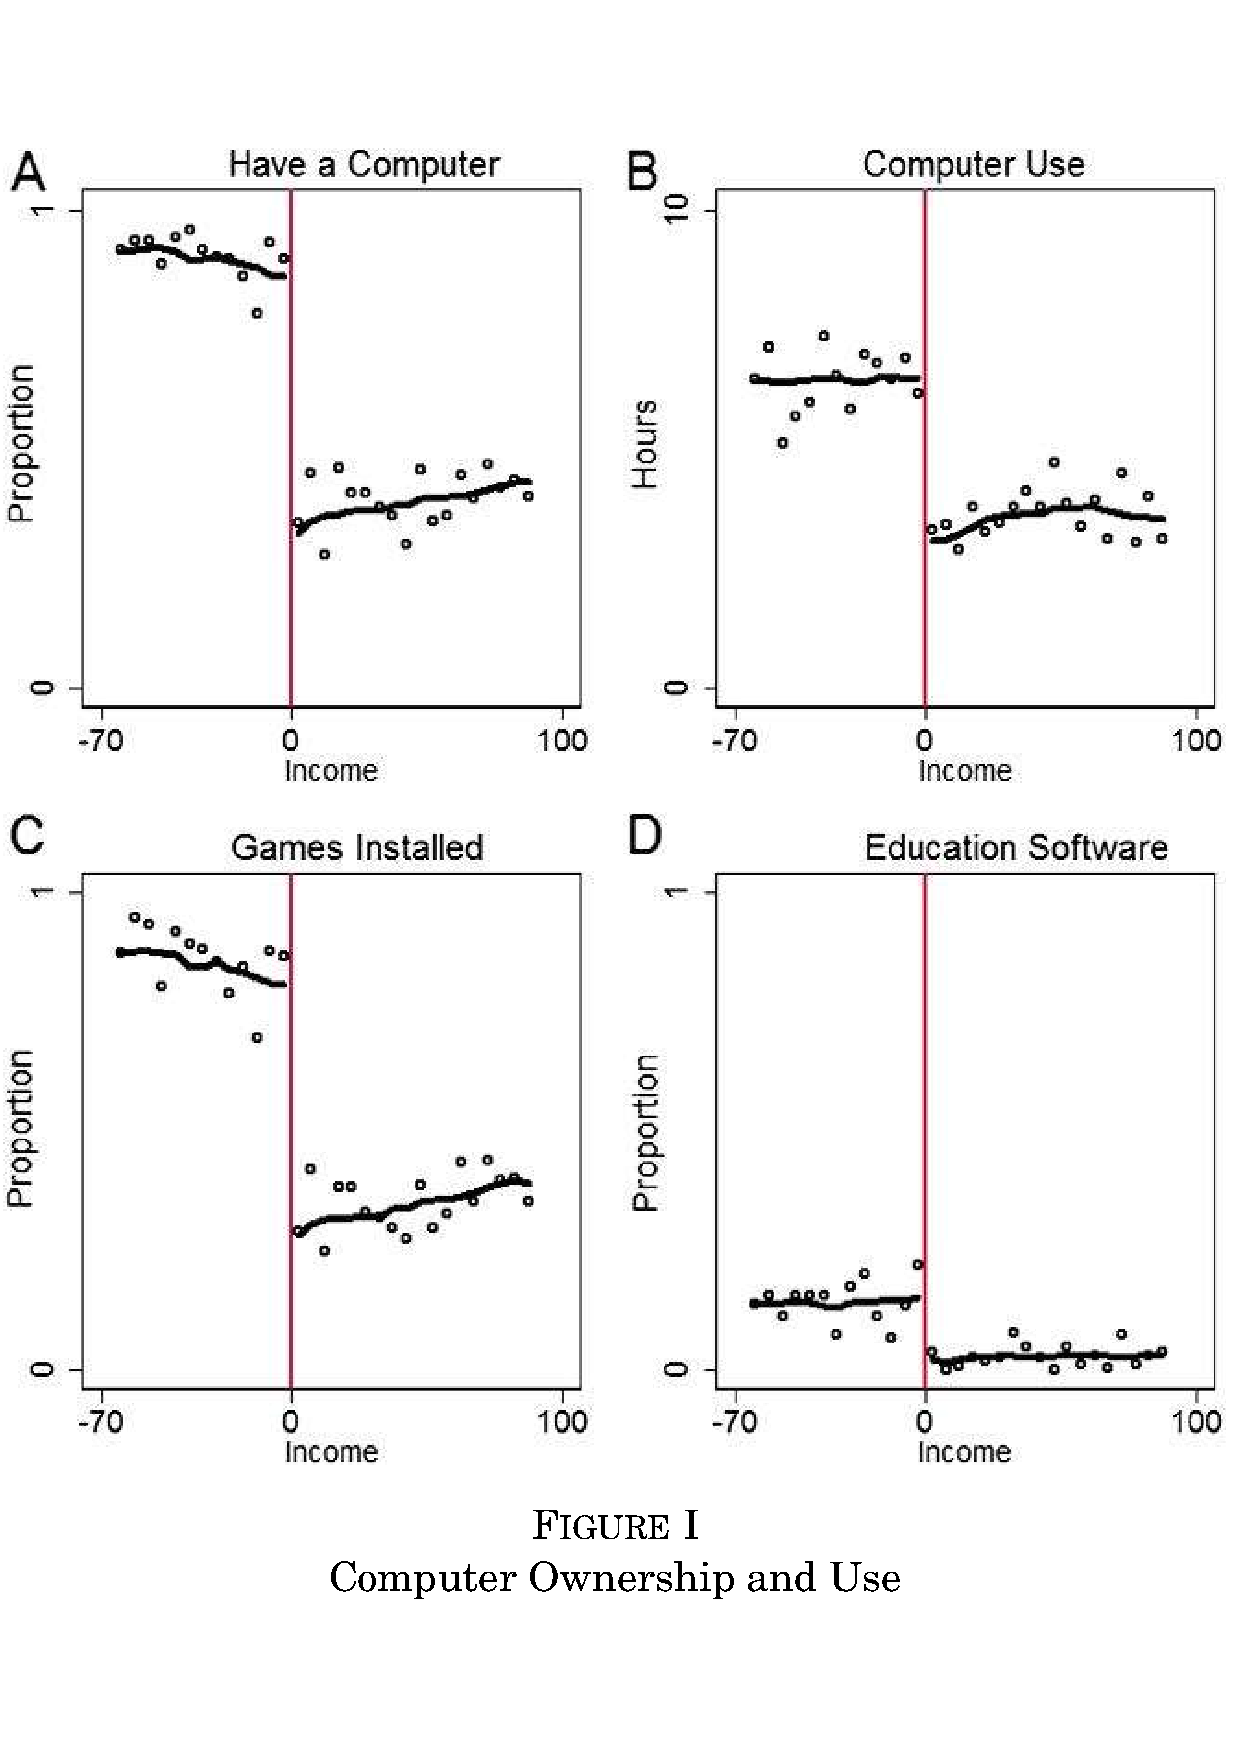
\includegraphics[width=0.4\textwidth]{fig1}
	\end{center}
\end{frame}
%------------------------------------------------
\begin{frame}[t]{Resultados}
	\begin{itemize}
	\item Los hogares que ganaron un voucher eran más de 50 ppt más propensos a tener una computadora en casa.
	\item Los/as niños/as en hogares que recibieron el cupón pasaron más horas por semana en la computadora: 2-4 horas. 
	\item Tener software educativo (12ppt) < juegos instalados (50ppt). 
	\item El cupón ganador no dio lugar a una diferencia significativa en el uso de Internet. 
	\end{itemize}
\end{frame}
%------------------------------------------------
\begin{frame}[t]{Resultados}
	\begin{itemize}
	\item 14 ppt más de probabilidades de usar una computadora para juegos a diario.
	\item Ganar un cupón no se tradujo en un mayor uso de la computadora para hacer la tarea.
	\item Ganar un cupón tiene un efecto negativo (significativo) en la lectura.
	\item El efecto sobre el uso del tiempo (en el televisor y en la tarea) puede estar sujeto a un error de medición (sesgo de recuperación).
	\end{itemize}
\end{frame}
%------------------------------------------------
\begin{frame}[t]{Resultados}
\begin{itemize}
\item Ganar un cupón tiene efectos negativos (significativos) en los logros académicos en matemáticas, rumano, inglés.
\item No hay efecto en comportamiento escolar. 
\item Los/as niños/as en hogares que recibieron un cupón tendían a tener puntuaciones de Raven significativamente más altas, pruebas de computadora, capacidad para operar una computadora y usar efectivamente la aplicación de computadora 		
\end{itemize}
\end{frame}
%------------------------------------------------
\begin{frame}[t]{Resultados}
Ahora, ¿qué pasa cuando existen reglas? 
\begin{itemize}
	\item Regulación del uso de la computadora → Reduce el tiempo dedicado a la computadora y la puntuación de la prueba de computadora, pero no mejora el GPA escolar. 
	\item Regulación de las actividades de tarea → Aumente el tiempo dedicado a la tarea y el GPA, y no disminuye las habilidades informáticas.
	\item Regulación en las actividades de tarea tienen un efecto más deseable que en el uso de la computadora. 
\end{itemize}
\end{frame}
%------------------------------------------------
\begin{frame}[t]{Conclusiones}
	\begin{itemize}
	\item El acceso a la computadora en el hogar tiene efectos positivos y negativos en el capital humano de los/as niños/as.
	\begin{itemize}
		\item Positivo: Mejora habilidades de computación y cognitivas. 
		\item Negativo: Empeora rendimiento académico. 	
	\end{itemize}
	\item A pesar de los esfuerzos del Ministerio de Educación de Rumania, pocos niños utilizaron su computadora con fines educativos. En cambio, las computadoras se utilizaban principalmente para jugar juegos.
	\item La participación y supervisión de los padres pueden ser factores mediadores importantes.
	\end{itemize}
\end{frame}
%------------------------------------------------
\section{Anuncios}
\subsection{Anuncios}
%------------------------------------------------
\begin{frame}{Anuncios}
\textbf{Taller en formato de discusión: }
\begin{itemize}
	\item Van a leer el paper de Palacios (2019) y responderán 5 preguntas generales sobre el tema.
	\item Utilizaran los mismos grupos del ensayo grupal. 
	\item El paper se encuentra en la plataforma del EVA. 
	\item Las preguntas las subiré mañana. 
	\item Fecha máxima de entrega: Lunes 15 de julio 6 pm. 
\end{itemize}
\end{frame}
%==============================================================
% END
%==============================================================
\miniframesoff 	
\begin{frame}[plain, standout]
Nos vemos la siguiente semana. 
\end{frame}
%------------------------------------------------
\end{document}		
